\capitulo{4}{Desarrollo y Modificaciones de la Arquitectura}

En este capítulo, se presentan los desarrollos principales que se han llevado a cabo durante el trabajo, prestando especial atención a las modificaciones realizadas sobre la arquitectura DPT.

\section{Cloud}\label{cloud}

Con el objetivo de reducir el tiempo necesario para entrenar los distintos modelos que se plantean en este trabajo, se ha recurrido al servicio de infraestructura (IaaS - \textit{Infraestructure as a Service}) que ofrece la empresa Google: Google Cloud. Los servicios en la nube (\textit{cloud}), permiten disponer de recursos informáticos de manera flexible, pagando únicamente por aquellos que estén activos. Los proveedores de IaaS, se encargan del mantenimiento y gestión de la infraestructura (redes, almacenamiento, servidores, virtualización), mientras que el usuario se encarga de la gestión del sistema operativo y todo lo que hay por encima. 

Dentro de Google Cloud, se han empleado los servicios \textbfit{Compute Engine}, para disponer de máquinas virtuales y \textbfit{Cloud Storage}, para crear recursos de almacenamiento (\textit{buckets}).

El flujo de trabajo que se ha seguido ha sido el siguiente (\Cref{fig:cloud-diagram}):

\begin{enumerate}
\item Primero, se ha creado un \textit{bucket} en el que se han dejado disponibles el conjunto de datos empleado durante el entrenamiento, el código necesario para ejecutar el entrenamiento, y una serie de scripts para facilitar la configuración del equipo. Al disponer de estos archivos en la nube, se desacoplan totalmente la configuración de las máquinas virtuales y el ordenador local en el que se lleva a cabo el desarrollo (Equipo 1 en \Cref{tab:computer-specs}).
\item A continuación, se configura una máquina virtual con el \textit{hardware} elegido\footnote{Para elegir el \textit{hardware} de las máquinas virtuales, se ha elegido la GPU que mayor relación TFLOPS/euro ofrecía para minimizar el coste de los equipos. El resto de características se han elegido de forma que la limitación del equipo sea el procesamiento en GPU.} (Equipo 2 en \Cref{tab:computer-specs}). Una vez conectados a esta máquina virtual a través de SSH, se descarga del \textit{bucket} creado el script de configuración (disponible en el \Cref{documentacion}) y se ejecuta. Este script, se encarga de: descargar el resto de archivos disponibles en el \textit{bucket}, instalar los drivers de NVIDIA necesarios para poder usar la GPU de la instancia, instalar Docker y el NVIDIA Container Toolkit, instalar Weights and Biases, y construir la imagen de Docker especificada en el Dockerfile descargado.
\item Una vez configurada la instancia con todos los archivos necesarios en su disco SSD, se crea una imagen de dicha instancia en Google Cloud de forma que sea fácilmente replicable. Posteriormente, se configura desde la consola de Google Cloud el inicio de estas instancias de forma que cada vez que se encienda una (nueva o ya existente), se cree dentro del equipo un contenedor de Docker a partir de la imagen ya construida, y se ejecute en este contenedor el cliente de Weight and Biases para entrenar modelos automáticamente. De esta forma, para añadir una nueva máquina al proceso de entrenamiento de experimentos, solamente hay que crear un nuevo equipo a partir de la imagen preconfigurada.
\item Por último, una vez finalizados los experimentos, se copian a través de SSH los parámetros de los modelos entrenados guardados en cada una de las máquinas virtuales empleadas.
\end{enumerate}

\begin{figure}[H]
\centering
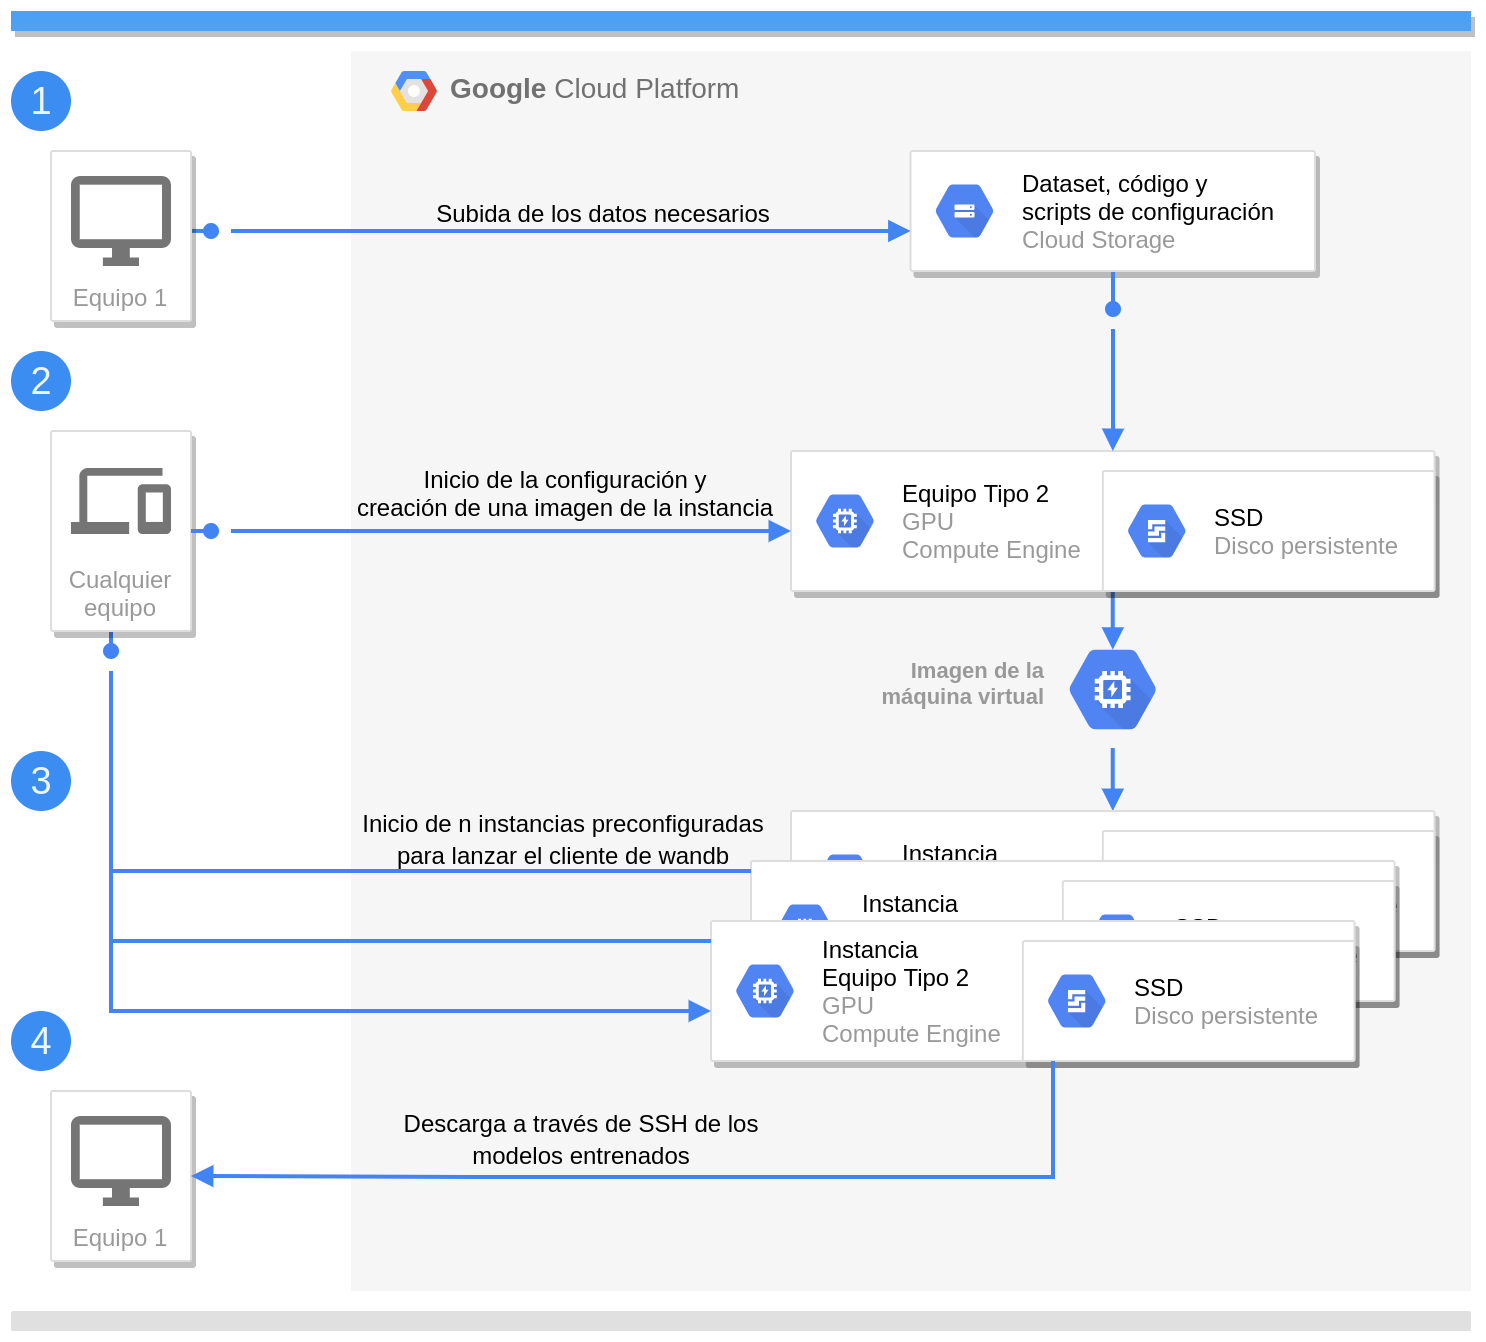
\includegraphics[width=\textwidth]{imagenes/cloud-diagram.png}
\caption{Esquema de la configuración llevada a cabo en la nube.}
\label{fig:cloud-diagram}
\end{figure}

\section{Warmstart}
Para acelerar lo máximo posible la convergencia del modelo durante el entrenamiento, se aprovechan en la medida de lo posible parámetros con sesgos inductivos ya aprendidos, es decir, parámetros de modelos ya entrenados. Más concretamente, los parámetros de los modelos a entrenar se inicializan con los valores de los parámetros del modelo DPT-Hybrid entrenado en MIX6, publicados en el artículo original de \textit{Dense Prediction Transformers} \cite{visiontransformersDPT}. 

Además, ya que en este trabajo se estudian diferentes modificaciones de dicho modelo, se emplea el método \texttt{load\_state\_dict()} de la clase \texttt{torch.nn.Module} con el parámetro \texttt{strict=False} para cargar los parámetros, evitando así que la carga falle si no coinciden una a una las capas en el modelo y las definidas en el archivo que se trata de cargar. En cuanto a las capas/conjuntos de capas que se han modificado y/o añadido, al no disponer del conjunto de datos MIX6 para preentrenarlas, se han inicializado con sus parámetros correspondientes tras ser entrenadas en ImageNet21K.

Esta forma de proceder, sin embargo, conlleva que los modelos con menor porcentaje de su arquitectura modificada partan de una situación inicial ventajosa para la tarea de estimación de profundidad monocular (al estar ya preentrenados en MIX6 en vez de ImageNet).

\section{Entrenamiento}
Pese a que los autores del artículo de DPT \cite{visiontransformersDPT} han publicado el código del modelo y sus pesos preentrenados en MIX6 y KITTI, a día de hoy no han hecho públicos los \textit{scripts} de entrenamiento empleados. Por esto, ha sido necesario escribir el proceso de entrenamiento así como el \texttt{Dataset} de PyTorch con el que leer los datos de KITTI.

Para el \texttt{Dataset}, se crea una clase \texttt{KITTIDataset}\footnote{\url{https://github.com/guillesanbri/DPT/blob/v1.0.0-tfm/KITTIDataset.py}} que hereda de la clase abstracta base para conjuntos de datos que ofrece PyTorch, \texttt{torch.utils.data.Dataset}, y sobreescribe los métodos \texttt{\_\_len\_\_()} y \texttt{\_\_getitem\_\_()} de forma que estos se adapten a la estructura de directorios y nombres de las imágenes y de sus anotaciones. Al sobreescribir estos métodos, es posible crear un \texttt{torch.utils.data.Dataloader} de forma directa, pasando las imágenes y las etiquetas a los modelos aprovechando las herramientas de PyTorch. En el método \texttt{\_\_getitem\_\_()}, además, se aplican las transformaciones necesarias a los datos, así como el \textit{Data Augmentation}.

Por \textit{Data Augmentation} se entiende el conjunto de operaciones y transformaciones que se pueden aplicar a los datos para modificar su apariencia. Esto normalmente favorece el aprendizaje y la capacidad de generalización de la red (tiene efecto regularizador y evita el sobreajuste al aumentar el número de ejemplos y la variedad entre ellos). En el entrenamiento llevado a cabo, siguiendo una vez más la metodología de DPT, se ha incluido un \textbf{reflejado horizontal aleatorio}, es decir, cada una de las imágenes (junto con las anotaciones) tiene un $50\%$ de posibilidades de ser reflejada horizontalmente antes de atravesar la red como ejemplo de entrenamiento.

En cuanto al \textit{script} de entrenamiento\footnote{\url{https://github.com/guillesanbri/DPT/blob/v1.0.0-tfm/train.py}}, se tienen en cuenta una serie de factores para acelerar el proceso lo máximo posible:
\begin{itemize}

\item \textbf{Número de trabajadores en el \texttt{Dataloader}}: Con el objetivo de asegurar que la limitación en la velocidad de entrenamiento sea el procesamiento en la GPU, se cambia el valor del parámetro \texttt{num\_workers} del constructor del \texttt{Dataloader} de entrenamiento a 8. Este parámetro, controla el número de procesos que se lanzan en paralelo para leer los datos del disco y preprocesarlos.

\item \textbf{\texttt{pin\_memory}}: También en el constructor del \texttt{Dataloader} es posible activar \texttt{pin\_memory}, parámetro desactivado por defecto. Este parámetro, acelera la transferencia a la memoria de la GPU de los datos cargados en memoria (RAM) por la CPU \cite{harris2012}. De forma resumida, lo que habilita este parámetro es que la carga de datos se haga en memoria no paginable (\textit{pinned}) a la que la GPU accede directamente, evitando así cargar los datos en una zona de memoria paginable y transferir estos a una \textit{pinned memory} temporal cada vez que la GPU quiere leerlos para transferirlos a su propia memoria.

\item \textbf{\texttt{torch.backends.cudnn.enabled y \texttt{torch.backends.cudnn.benchmark}}}: Estas dos opciones, se activan para asegurar, respectivamente, que se use CuDNN en la ejecución del modelo y que se ejecuten al comienzo del \textit{script} distintas implementaciones de algoritmos de convolución para emplear el más rápido en el sistema actual.

\item \textbf{\textit{Mixed precision}}: Ya mencionado en el \Cref{optimizacion-modelos}, pese a que finalmente se ha descartado su uso en el entrenamiento debido a la inestabilidad numérica que introducía y los fallos que ocasionaba, el \textit{script} de entrenamiento incluye la opción de activar el uso de precisión mixta con el escalado pertinente.
\end{itemize}

Para ajustar los parámetros de los modelos, se ha empleando como optimizador \texttt{AdamW} con una tasa de aprendizaje $lr = 1e-5$ y parámetros: $\beta_1 = 0.9$, $\beta_2 = 0.999$, $\epsilon = 1e-8$ y $\textit{weight decay} = 0.01$. El número de épocas se ha fijado en $20$ tras analizar el comportamiento de la pérdida en distintas ejecuciones previas. En cuanto al tamaño de lote usado, se ha utilizado solamente una imagen para cada actualización de parámetros. Esta elección viene motivada por dos razones, la primera, la falta de recursos computacionales para entrenar algunas de las variaciones de los modelos con lotes de más imágenes, y la segunda y más importante, que tras implementar en el \textit{script} de entrenamiento la posibilidad de acumular gradientes\footnote{La acumulación de gradientes (\textit{gradient accumulation}) es una técnica que promedia las pérdidas en distintos lotes para, aún sin poder aprovechar la mejora de rendimiento de un tamaño de lote mayor, conseguir que la actualización de los parámetros sea matemáticamente equivalente (con alguna limitación como la imposibilidad de usar \textit{batch normalization}) a usar un tamaño de lote mayor.}, se comprobó que se obtenían mejores resultados con lotes de una sola imagen, probablemente por el efecto regularizador característico de un tamaño de lote tan reducido.

Además, se ha empleado la función \texttt{torch.nn.utils.clip\_grad\_value\_}, que se encarga de limitar los valores de los gradientes en función de su valor con un \texttt{clip\_value} de $0.5$, limitando considerablemente las posibilidades de que explotasen los gradientes del modelo y se desestabilice su entrenamiento. No obstante, como precaución y para evitar el desperdicio de recursos, el entrenamiento se detiene en caso de que el valor de la función de pérdida se vuelva $\pm \infty$.


\subsection{Función de pérdida}
La función de pérdida usada durante el proyecto, y por lo tanto implementada en el script de entrenamiento, es la función empleada en la publicación de DPT \cite{visiontransformersDPT} para ajustar los modelos preentrenados en MIX6 a \textit{datasets} más pequeños. Tal y como indica esta publicación, su función de pérdida se compone de la función de pérdida propuesta por Eigen et al. \cite{eigen-multi-scale} y de otra función que calcula los gradientes de la profundidad obtenida para penalizar la falta de suavidad en píxeles contiguos, propuesta en el trabajo de Li et al. \cite{MegaDepthLi18}. No obstante, como el \textit{dataset} empleado en este trabajo es KITTI y sus anotaciones son dispersas, no es posible calcular dichos gradientes en las etiquetas y por lo tanto se elimina esa parte de la función. 

De esta forma, la función de pérdida resultante es la definida por la \Cref{eqn:perdida-midas}, donde $\hat{d_p}$ es la profundidad obtenida de la red para cada píxel $p$, $d_p$ es la etiqueta con los valores de profundidad, $n$ es el número de píxeles que tienen un dato de profundidad en la etiqueta correspondiente y $\lambda$ es un hiperparámetro cuyo valor puede estar en el rango $[0, 1]$ y controla la influencia de la escala, ya que con $\lambda=0$ el segundo término se anula (quedando la distancia de cuadrados en espacio logarítmico), y con $\lambda=1$ la función de pérdida es invariante a la escala. La demostración de la invariancia a la escala es equivalente a la de la métrica \textit{SIlog} (\Cref{demostracion}), ya que dicha métrica es la raíz cuadrada de esta función de pérdida. Para el entrenamiento de los modelos, $\lambda$ se ha fijado en $0.5$.

% di = torch.log(masked_output) - torch.log(masked_target)
% n = masked_output.shape[0]
% di2 = torch.pow(di, 2)
% fisrt_term = torch.sum(di2) / n
% second_term = 0.5 * torch.pow(torch.sum(di), 2) / (n ** 2)  0.5 is lambda
% loss = fisrt_term - second_term
% return loss.mean()
\begin{equation}
\label{eqn:perdida-midas}
L(\hat{d}, d) = \frac{1}{n}\sum_{p} (\ln{\hat{d_p}} - \ln{d_p})^2 - \frac{\lambda}{n^2} \left( \sum_{p} (\ln{\hat{d_p}} - \ln{d_p}) \right)^2
\end{equation}

\section{Modificaciones introducidas en DPT}
En esta sección se describen las distintas modificaciones y desarrollos que se han introducido en la arquitectura original de DPT a lo largo del proyecto, y que por lo tanto, conforman las distintas variantes del modelo que se entrenarán y evaluarán.

\subsection{Reducción de tamaño de la entrada}
Para acelerar DPT lo primero que se modificó fue el tamaño de la entrada, buscando estudiar la flexibilidad de la arquitectura para aprender a inferir profundidad a partir de imágenes con menor resolución. Los resultados de la publicación original calculan la profundidad en el conjunto de evaluación de KITTI con las imágenes en su tamaño original, 1216x352. Para reducir el consumo de memoria del modelo durante su entrenamiento, así como acelerar entrenamiento e inferencia, se han añadido dos operaciones de cambio de tamaño: una al principio de la red que reduce el tamaño de las imágenes a 640x192 píxeles, y otra al final de la red que reescala la salida al tamaño original. 

% La primera operación emplea como método de interpolación el algorítmo \texttt{INTER{\_}AREA} de OpenCV, que TODO y está recomendado para reducir el tamaño de imágenes ya que proporciona resultados sin efecto Moire; la operación que amplia la salida al tamaño de la imagen original, por otro lado, emplea interpolación bicúbica.

% \todo[inline]{Explicar inter{\_}area, citarlo? explicar en una nota al pie qué es el efecto moire?}

% https://medium.com/@wenrudong/what-is-opencvs-inter-area-actually-doing-282a626a09b3

\subsection{Capas de atención eficiente}

Tal y como se ha visto en el \Cref{atencion-eficiente} de Marco Teórico y Estado del Arte, existen numerosas técnicas para reducir la complejidad computacional y requisitos de memoria de los mecanismos de atención característicos de los \textit{transformers}. Sin embargo, estas técnicas ofrecen mayores incrementos en el rendimiento cuanto mayor es la longitud de la cadena de la entrada. Por lo tanto (especialmente tras reducir el tamaño de las imágenes) no se va a apreciar un incremento especialmente substancial en la velocidad de inferencia por modificar estos mecanismos. Aún así, se decide modificar el mecanismo de atención con el objetivo de estudiar la capacidad de estas nuevas técnicas para igualar los resultados de los mecanismos originales. En concreto, se compara el mecanismo de atención del \textit{Perfomer} con la atención estándar.

Para poder llevar a cabo los experimentos relacionados con este aspecto de la arquitectura y poder entrenar los modelos necesarios, se modifica el código de DPT de forma que se puedan seleccionar distintos mecanismos de atención, entre ellos la implementación del mecanismo de atención del \textit{Performer} desarrollada por Phil Wang \cite{pwperformer}. Entre los distintos mecanismos de atención eficiente, se ha elegido el del \textit{Performer} debido a que tiene una complejidad $O(n)$ y también debido a que, según apuntan los autores en su publicación, es posible reutilizar los parámetros de las matrices de pesos $W^V$, $W^K$ y $W^Q$ de los mecanismos de atención estándar para obtener las matrices $Q$, $K$ y $V$ (hace falta un pequeño ajuste, pero no es necesario entrenar desde cero).

\subsection{Número de cabezas}
En la publicación \textit{Are Sixteen Heads Really Better than One?} \cite{are16headsbetterthan1}, se plantea y prueba la idea de que el número de cabezas en los bloques de atención está sobredimensionado, siendo posible eliminar un gran porcentaje de las cabezas sin afectar al rendimiento de forma significativa. Esta influencia en el rendimiento, se reduce aún más cuando se reentrena el modelo después de reducir el número de cabezas.  Además, los autores señalan que reducir el número de cabezas degrada el rendimiento de forma más significativa en los bloques de \textit{Cross-Attention} (\Cref{bloques-atencion}) con elementos del \textit{encoder} y \textit{decoder} que en los bloques de \textit{Self-Attention}. 

En el caso de DPT, al emplear como \textit{encoder} un ViT, no existen bloques de \textit{Cross-Attention}, si no que son todos de \textit{Self-Attention} (recordemos que el ViT solo se compone de la parte del \textit{encoder} del \textit{transformer} original). Por lo tanto, se plantea también como una de las modificaciones del proyecto estudiar la influencia del número de cabezas en la velocidad de inferencia y los resultados, adaptando el código del modelo para que sea posible cambiar la cantidad de cabezas en los bloques de atención (tanto de atención estándar como de atención eficiente). Los valores con los que se experimenta para este hiperparámetro son $1$, $12$ (el número de cabezas que tiene DPT por defecto) y $24$.

\subsection{Hooks del transformer y bloques de atención posteriores}

En la arquitectura de DPT (\Cref{DPT}), la transferencia de información desde el \textit{encoder} al \textit{decoder} tiene lugar a través de cuatro ganchos o \textit{hooks} que toman las salidas de ciertas capas para que pasen a ser las entradas que se fusionan en el \textit{decoder}. En la publicación original, si bien es cierto que se valoran diferentes tamaños de \textit{Vision Transformers}, no se presenta ningún experimento modificando los bloques de atención de los cuales se cogen las salidas. Más concretamente, el modelo DPT-Hybrid coloca dos de estos \textit{hooks} en el \textit{backbone} convolucional y los otros dos en los bloques de atención número 8 y número 11 (empezando en cero). Por lo tanto, la imagen de entrada tiene que atravesar todos los bloques de atención del ViT-Hybrid para conseguir la salida del último bloque de atención.

Los valores que se han probado en este trabajo para estos \textit{hooks} del ViT, es decir, los bloques de atención cuya salida se ha seleccionado como entrada del \textit{decoder}, son: bloques número 0 y 1, bloques número 2 y 5, y por último, bloques número 8 y 11 (siendo estos últimos los de la publicación original).

Al modificar las capas del transformer de las que se cogen las activaciones para pasarlas a la etapa de fusión convolucional, se abre la posibilidad de eliminar aquellos bloques de atención que ya no se usan. Por lo tanto, se ha modificado el código de la arquitectura para incluir dos cambios en el momento de instanciar el modelo: el primero, capar la inferencia para que la ejecución del ViT se detenga cuando llega al bloque de atención más alto requerido por los \textit{hooks}, y el segundo, eliminar las capas superiores no empleadas. De esta forma, además de acelerar el entrenamiento e inferencia del modelo, se reduce su tamaño considerablemente, tanto a la hora de almacenar sus parámetros como a la hora de cargarlo en memoria para desplegarlo en una aplicación real. 

En la \Cref{fig:attention_block_num} se puede apreciar la modificación del ViT empleado en DPT: a la izquierda está el \textit{encoder} tal y como se encuentra en el trabajo de DPT, con los \textit{hooks} en los bloques 8 y 11, sin eliminar ninguno de los parámetros del \textit{transformer}, y con la inferencia recorriendo los 12 bloques de atención; a la derecha, por otro lado, está una de las opciones valoradas para este hiperparámetro de la arquitectura, donde los \textit{hooks} se sitúan en la salida de los bloques 0 y 1 del ViT. De esta forma, en el ejemplo, los parámetros a partir del segundo bloque de atención se eliminarían ya que la inferencia del modelo solo llega hasta este segundo bloque.

\begin{figure}[H]
\centering
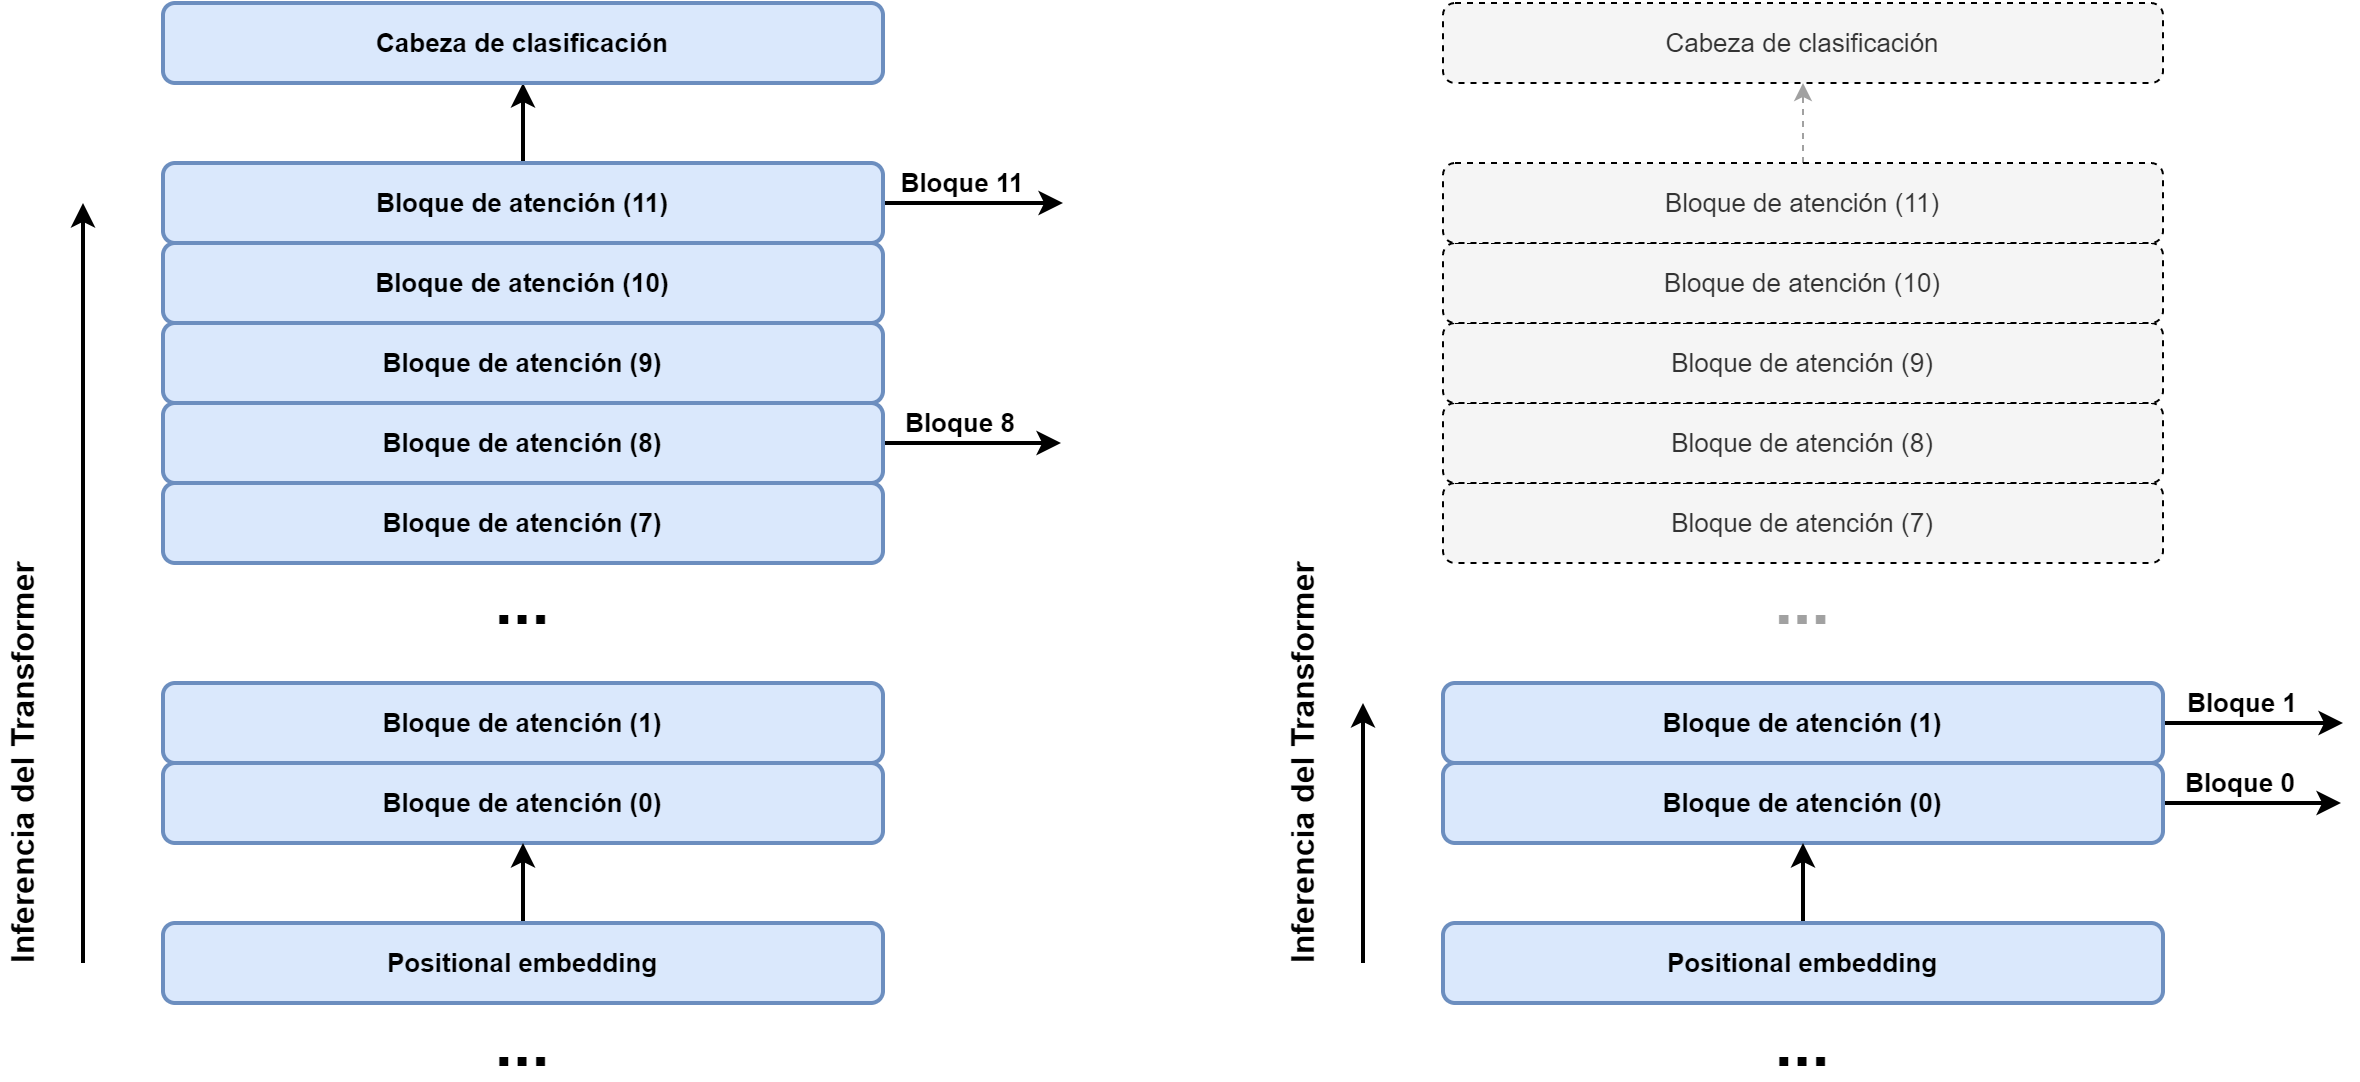
\includegraphics[width=\textwidth]{imagenes/DPT-cambio-bloques-transformer.png}
\caption{Cambio en los \textit{hooks} y en el número de bloques de atención.}
\label{fig:attention_block_num}
\end{figure}

\subsection{Backbone convolucional}
La última modificación de la arquitectura de DPT estudiada en este proyecto es la del \textit{backbone} convolucional del ViT-Hybrid, encargado de extraer los mapas de características empleados para obtener los \textit{tokens} que pasan a los bloques de atención. 

En el modulo propuesto en la publicación original, se elige como \textit{backbone} una ResNet50. De esta red, se extraen las activaciones en los bloques 0 y 1 para pasarlas al \textit{decoder}. Por otro lado, la salida de la última capa de la ResNet50, es decir, la entrada de los bloques de atención, tiene forma [n, c, h, w], donde: n es el número de imágenes en el lote (\textit{batch size}), c es el número de canales (en este caso mapas de características), y h y w la altura y anchura de los mapas de características. En el caso de este \textit{backbone}, la salida está compuesta por $c=1024$ mapas de características de dimensiones iguales a las de la imagen de entrada divididas 4 veces entre 2.

Después de la ResNet, hay una capa de proyección que no es más que una capa convolucional con \textit{kernels} de tamaño $1\times1$ y zancada $1\times1$, con $1024$ canales de entrada y $768$ canales de salida. Este tipo de convoluciones $1\times1$, realmente se componen de $786$ kernels de $1\times1\times1024$, por lo que al convolucionar cada uno de ellos con la entrada, se obtienen $768$ mapas de características del mismo tamaño que los de la entrada. Después, los $768$ mapas de características resultantes se aplanan en tensores de forma [$n$, $768$, $\frac{h}{8} \times \frac{w}{8}$] y se transponen de forma que la entrada sea de tipo [$n$, $t$, $768$], donde $768$ es el tamaño de los \textit{tokens} de los bloques de atención y t el número de \textit{tokens} extraidos de la imagen. De esta forma, a mayor tamaño de imagen mayor será el número de \textit{tokens} (secuencia más larga, aumenta el coste de los bloques de atención), pero la dimensión de estos permanece constante.

A modo de ejemplo, supongamos una entrada de una sola imagen de tamaño $384\times384$: la salida de la ResNet50 tendrá la forma [$1$, $1024$, $24$, $24$]. Esta salida atraviesa la convolución $1\times1$ de proyección y pasa a tener forma [$1$, $768$, $24$, $24$]. Estos mapas de características se aplanan en un tensor [$1$, $768$, $576$] que se traspone para obtener la forma [$1$, $576$, $768$], que equivale a $576$ \textit{tokens} de dimensión $768$. Una vez llegados a este punto, el tensor está listo para pasar a los bloques de atención del \textit{transformer}.

Buscando una alternativa que ofrezca resultados similares con un menor coste computacional, se adapta e incluye en las pruebas la arquitectura EfficientNet-B0 como \textit{backbone} convolucional de DPT. Esta arquitectura, proporciona una salida de forma [n, c, h, w] (manteniendo la nomenclatura anterior) donde el número de mapas de características es ahora $1280$ y la altura y anchura se corresponden con las de las imágenes de entrada divididas 5 veces entre 2. Es decir: [$n$, $1280$, $\frac{h}{16}$, $\frac{w}{16}$]. Para sustituir el \textit{backbone} convolucional del ViT-Hybrid sin tener que cambiar el tamaño de todas las capas de atención (y así aprovechar los pesos preentrenados), se sustituye la capa de proyección mencionada en el párrafo superior, que recordemos era una capa convolucional con kernels de tamaño $1\times1$ por una capa de convolución transpuesta. Esta capa de convolución transpuesta, cumple dos funciones fundamentales: la primera, proyectar los $1280$ mapas de características en $768$ gracias al número de \textit{kernels} empleados; y la segunda, al tener \textit{kernels} de tamaño $2\times2$ y una zancada también de $2\times2$, conseguir que las dimensiones de los mapas de características se multipliquen exactamente por $2$ en ambas dimensiones, convirtiendo la entrada [$n$, $1280$, $\frac{h}{16}$, $\frac{w}{16}$] en [$n$, $768$, $\frac{h}{8}$, $\frac{w}{8}$]. Estas dimensiones, son las que espera la etapa de \textit{embedding} que aplana los mapas de características y transpone el tensor para obtener la entrada de los bloques de atención, quedando a su salida un tensor con forma [$n$, $t$, $768$] donde $t$ vuelve a ser el número de \textit{tokens} que pasan al \textit{transformer}, cada uno de dimensión $768$.

Dado que no se disponen de los parámetros ajustados en MIX6 para EfficientNet-B0, se ha modificado también el \textit{script} del modelo para cargar en su inicialización los parámetros ajustados en ImageNet21K (proporcionados por la librería PyTorch Image Models \cite{timm}, de donde también se ha utilizado la implementación de EfficientNet-B0) correspondientes a este nuevo módulo. 

\section{Pruebas de cuantificación}
Además de las modificaciones comentadas, se han probado exhaustivamente distintos \textit{frameworks} de optimización y cuantificación. Más concretamente, se han probado los frameworks de optimización TensorRT (TRT) de NVIDIA y TF Lite, de TensorFlow. Para estas pruebas, se han utilizado tanto los modelos originales de PyTorch (en TensorRT) como los modelos convertidos a ONNX (ecosistema que permite la interoperabilidad entre \textit{frameworks} de aprendizaje profundo). Además de con TRT y TF Lite, se ha tratado de cuantificar el modelo tanto estática como dinámicamente empleando el cuantificador de PyTorch.

En el caso de los dos primeros \textit{frameworks} de optimización, no se ha conseguido ejecutar de forma exitosa la optimización de los modelos. La razón de los fallos obtenidos es que algunas de las capas de la arquitectura de DPT-Hybrid no están soportadas por la conversión de modelos, es decir, sería necesario ampliar las capacidades de las herramientas para implementar la optimización de dichas capas. Por otro lado, con el cuantificador de PyTorch tampoco se han conseguido resultados satisfactorios, en este caso, debido principalmente a la extracción de salidas intermedias del \textit{encoder} para pasarlas al \textit{decoder}, que ocasiona inconsistencias entre las operaciones que se llevan a cabo como enteros de 8 bits y como números en coma flotante de 32 bits.

Las dificultades encontradas al usar estos paquetes de \textit{software} son solucionables ampliando las funcionalidades de las herramientas. No obstante, este desarrollo no es trivial y excede el alcance de este Trabajo Fin de Máster. Por lo tanto, se propone su desarrollo como una posible línea de trabajo futuro.


% En los resultados hablar de la distribución de los pesos antes y después de convertir el modelo si es pertinente, hacer una especie de estudio de ablación si se puede entrenar modelos, etc. Puede estar interesante quitar cabezas de atención, quitar bloques de atención, ver como afecta al tamaño dle modelo, su rendimiento (velocidad y métricas)...

%\begin{figure}[H]
%\centering
%\includegraphics[width=\textwidth]{imagenes/DPT-modificado-general.png}
%\caption{Arquitectura general DPT tras las modificaciones.}
%\label{fig:dpt-mod-general}
%\end{figure}

\clearpage